\cleardoublepage
\chapter{Background and Related Work}
\label{cha:background}
The main contributions of this thesis revolve around the SimRa project (see \Cref{subsec:simra}), which is a crowdsourcing citizen science application, with the goal of revealing dangerous hotspots in bicycle traffic, that are detrimental to cycling safety and comfort.
This chapter provides an overview of the fundamental topics that are essential for a comprehensive understanding of the nature of the SimRa project and, consequently, the contributions outlined in \Cref{part:contributions}.
Research shows that feeling comfortable and safe while cycling go hand in hand.
Factors that make a cycling trip more comfortable also make it safer, and vice versa ~\cite{shoman2023evaluation, fitch2018relationship}.
For this, we first outline which factors mainly influence cycling comfort and give an overview of recent studies from that research area in \Cref{sec:cycling_comfort_background}.
We then continue with cycling safety in \Cref{sec:cycling_safety_background}.
There, we also differentiate between solitary and multi-participant accidents.
In \Cref{sec:crowdsourcing_crowdsensing_background}, we point out similarities and differences between crowdsourcing and crowdsensing, so that we can later, in \Cref{sec:simra}, better categorize the SimRa project.
The last topic we look into, is the field of citizen science, namely what makes a project a citizen science project, which benefits and challenges it brings, and how the related work uses it in \Cref{sec:citizen_science_background}.
We conclude this chapter with a summary in \Cref{sec:summary_background}.

\section{Cycling Comfort}
\label{sec:cycling_comfort_background}
According to surveys, a low level of cycling comfort is one of the main reasons why people choose other modes of transportation, especially driving a car, over cycling.
This issue underlines the importance of cycling comfort when trying to increase the modal share of cycling.
The Cambridge Dictionary\footnote{https://dictionary.cambridge.org/} defines comfort as
``a pleasant feeling of being relaxed and free from pain''.

According to that definition, a comfortable ride needs to be absent of both \textit{mental} and \textit{physical} stress factors.
Related work has identified four factors that can cause mental and physical strain on the cyclist: cycling posture, cycling smoothness, environment, and mental state.

\subsection*{Cycling Posture}
A wrong cycling posture does not only result in lower cycling comfort, but it can also cause medical problems, especially over long periods of time, such as painful pelvic bones or pain in the region of the
perineum~\cite{christiaans1998comfort}.
Causes for a wrong cycling posture can be a wrong-sized bicycle frame, a misaligned handlebar, or a saddle that is too high, too low, or badly angled.
The shape of the saddle as well as the handlebar are also important, as different types of saddle and handlebars result in different cycling postures~\cite{bressel2003bicycle}.
Informing cyclists about the importance of cycling posture, so that they can buy the right bicycle for them, as well as adjust the bicycle they already have, seems to be a good way to improve the cycling postures of cyclists and thus increase their cycling comfort.

\subsection*{Cycling Smoothness}
Vibrations stemming from the rolling of the bicycle wheels on the surface can also lead to a decrease in comfort.
These vibrations are mainly conducted to the cyclist through the contact points with the bicycle, usually at the handlebar and the saddle.
This means, that if the handlebar and the saddle absorb the vibrations of the ride, the cycling will be more smooth and thus more comfortable for the cyclist.
The use of soft materials or effective suspensions, in conjunction with high-quality, vibration-absorbing tires, can contribute to a more comfortable ride.
However, the road surface itself represents the most significant factor:
Without a well-constructed and well-maintained infrastructure, even the most advanced bicycle will be unable to fully absorb the vibrations caused by uneven surfaces, cracks, and potholes in a poorly maintained bicycle lane or road.

\subsection*{Environment}
The environment is a significant factor that influences the comfort level of a cycling trip~\cite{hull2014bicycle}.
Thereby, we can distinguish between the \textit{natural} and the \textit{built} environment.
Climate, weather, scenery, and topography belong to the \textit{natural} environment.
For the majority of cyclists, inclement weather, including strong winds, precipitation, low temperatures, and high temperatures combined with humidity~\cite{nkurunziza2012examining}, is a significant impediment to their comfort while cycling.
The study by Boyce et al.~\cite{boyce2000perceptions} shows that people feel more comfortable during the daytime, so long winters with short daytimes, as is common near the poles, also lead to less comfortable cycling trips.
Wessel et al.~\cite{wessel2022cycling} look further into this issue and find out, that adopting daylight saving time throughout the year would increase the amount of cycling.
A nice scenery along the cycling trip route can increase cyclist satisfaction and thus result in a higher comfort level~\cite{wahlgren2012exploring,willis2013uniquely}.
While hills can be advantageous for recreational cycling trips due to the nice scenery and the physical effort to cycle up to a hill, which is commonly sought after by recreational cyclists, they are often perceived as a nuisance by commuting cyclists~\cite{lee2008neighbourhood}.

So the \textit{natural} environment can impact the comfort of a cycling trip both in positive and negative ways.
Similarly, the \textit{built} environment can further enhance the positive and negative effects of the \textit{natural} environment.
As the name suggests, the \textit{built} environment refers to environmental circumstances realized by humans.
The most obvious one to mention here is the bicycle infrastructure.
Not only does a well-planned and maintained bicycle infrastructure reduce unpleasant vibrations and bumps during the cycling trip, but it also contributes to a comfortable ride by making clear how the cyclist has to behave in traffic, e.g., when approaching an intersection.
A well-maintained infrastructure is also important for mitigating the downsides of bad weather, especially the removal of accumulated snow on bike lanes/paths is crucial~\cite{an2019weather,shoman2023evaluation}.
Likewise, street lights illuminating the bicycle infrastructure lead to a more comfortable cycling trip, because it makes it easier for the cyclist to perceive the surroundings and avoid potential hazards~\cite{digioia2017safety}.

In general, physical well-being and a feeling of safety are important factors for comfortably cycling, which is why the next section deals with cycling safety.
  

\section{Cycling Safety}
\label{sec:cycling_safety_background}
A (perceived) lack of safety is one of the main factors why potential cyclists prefer other modes of transportation over cycling~\cite{felix2020build,nazemi2021studying,lawson2013perception}.
Hence, it is important to understand what increases or decreases the (perceived) safety of cycling and how to make cycling safer, both objectively and subjectively.
The emphasis on perceived/subjective safety is important in two ways:
On one hand, if the perceived safety of a road segment is higher than the objective safety, cyclists are not aware of the risk they put themselves in~\cite{christ2023perceiving}.
On the other hand, when the safety of cycling is perceived to be lower than it actually is, potential cyclists stay away from cycling due to a misconception~\cite{noland1995perceived}.

First, we look into the objective safety in bicycle traffic, before we highlight the issues regarding perceived safety.
The main safety concern regarding cycling safety is accidents.
These can be differentiated into two categories:  solitary accidents, such as falling from the bike due to losing balance or slipping in winter conditions, and multi-participant accidents.

\subsection*{Solitary Accidents}
In their studies, Juhra et al. and Naess et al. investigate bicycle accidents, that were not reported to the police by analyzing hospitalization reports, where the patient was admitted after a bicycle accident~\cite{juhra2012bicycle,naess2020number}.
This is a good way to study solitary accidents since these are usually not reported to the police.
Solitary accidents make up the majority of bicycle accidents~\cite{juhra2012bicycle,naess2020number} and the most common form is falling from the bicycle without external forces.
Reportedly, most of these accidents happen to young and middle-aged adults during rush hours, which correlates with increased bicycle traffic activity during these times.
Interestingly, children, probably due to their inexperience, and the elderly, probably due to the tolls of age on the human body, experience much more solitary accidents than multi-participant accidents.
Better bicycle infrastructure, i.e. well maintained and well-lit bicycle roads, especially during winter, is needed to decrease the risk of falling from the bicycle without external forces since they likely happen due to bumps in the road that were seen too late to circumvent by the cyclists or due to black ice.
Another interesting finding is, that at nighttimes the cyclists, who fall from the bicycle without external forces are young adults, probably returning from partying, thus raising awareness could also decrease this type of accident.

Other types of solitary accidents are collisions with fixed objects, such as trees, or accidents caused by a technical defect of the bicycle.
Statistics about collisions with fixed objects are very similar to falling from the bicycle without external forces, which further supports the above-mentioned causes and proposed solutions.
Especially younger people such as students tend to have cheaper bicycles due to their lower income and fear of their bicycles getting stolen.
Cheap and old bicycles are more susceptible to technical defects, which is probably why younger people have more accidents caused by them.
More awareness and easier access to bicycle (self-)repair stations could mitigate this problem.

\subsection*{Multi-Participant Accidents}
The predominant form of traffic crashes in bicycle traffic are accidents with motorized vehicles~\cite{juhra2012bicycle,naess2020number}.
Similar to solitary accidents, multi-participant accidents mostly happen to young and middle-aged adults during rush hours.
This is no surprise since these are also the times with the biggest motorized vehicle traffic volumes, which lead to a bigger exposure of cyclists to motorized vehicle traffic.
In contrast to solitary accidents, multi-participant accidents happen more during the daytime.
The fact that there is more traffic during daytime in general and that motorized vehicle drivers drive more carefully, when the view is impaired, e.g., by darkness or bad light conditions~\cite{schepers2011road}.
It is also worth noting, that multi-participant accidents usually result in more serious injuries and mortality than solitary accidents. 
These findings stress the necessity for a separation of bicycle and motorized vehicle traffic with physically separated bicycle tracks since these reduce the risk of a crash between them by at least 50\%~\cite{van2021safety}.

\subsection*{Near Miss Incidents}
Aldred and Crossweller define \textit{near miss incidents}\footnote{In the remainder of this thesis, we will also refer to them as ‘‘incidents’’.} as non-injury accidents that can be frightening and/or annoying~\cite{aldred2015investigating}.
Consequently, incidents can be regarded as multi-participant accidents, wherein a collision between the cyclist and the other participant is either averted or is so mild, that neither the participants, nor their belongings sustain any harm.

Incidents can be classified into one of the following eight categories:~\cite{aldred2015investigating,aldred2016cycling,aldred2018predictors}
Close Pass, someone pulling in or out, near left/right hook, someone approaching head-on, tailgating, near-dooring, dodging an obstacle, and “other”.
Nevertheless, even if such incidents do not result in injuries or fatalities, they are still detrimental for the well-being of cyclists and by extension, to that of society as a whole.
Incidents, particularly those perceived as ‘‘very scary’’ by the cyclists, can induce stress, which may contribute to a detrimental mental state and an increased risk of developing further illnesses.~\cite{yaribeygi2017impact}.
Additionally, prospective cyclists may be dissuaded by the prospect of injury, which incidents may exacerbate.~\cite{aldred2015investigating}.

Two main approaches can be taken to prevent incidents: infrastructural and behavioral changes.
The former involves physically separating cycling traffic from motorized vehicle traffic, for example, by installing metal or concrete barriers between the car and cycling lanes.
The latter can be achieved through educational campaigns can be started to improve the driving behavior of motorized vehicle drivers.
Additionally, the existing laws, that should prevent incidents, such as close passes, could be enforced more rigorously and strictly. 

%\subsection*{Bicycle Helmets}
%TODO

\section{Crowdsourcing and Crowdsensing}
\label{sec:crowdsourcing_crowdsensing_background}
Crowdsourcing and crowdsensing have emerged as successful approaches for solving tasks in a fast and cost-efficient way and gathering big amounts of data in a short time respectively.

\subsection*{Crowdsourcing}
``Crowdsourcing'' is a combination of the words \textit{crowd} and \textit{outsourcing}~\cite{howe2006rise}.
\textit{Crowd} refers to an often large group of individuals, to which a task is transferred, whereas outsourcing refers to a practice where an entity does not fulfill a task in-house on its own, but hires people from outside to solve a task for them.
Crowdsourcing comes in many shapes and forms and can be found in many different areas, from transportation to financing, from social media to natural crisis relief, etc.
A very common form of crowdsourcing is the so-called mobile crowdsourcing.
In mobile crowdsourcing the people fulfilling the task usually do not have to be stationary, but rather mobile, because the task at hand demands movement or being in a specific location to be fulfilled~\cite{phuttharak2018review}.
In the latter case, a smartphone or a hardware device fitted with sensors has to be used by the participants to fulfill the task.
For the remainder of this work, we will use the terms crowdsourcing and mobile crowdsourcing interchangeably.

Figure~\ref{fig:crowdsourcing_architecture} shows the key elements of crowdsourcing.
In the top layer, the application user (e.g., a ride-hailing app user) requests a task (e.g., a trip from location A to location B).
The data processing platform layer receives this task and determines to whom (e.g., which taxi drivers) to allocate it.
Then, the crowd (e.g., the taxi driver, that accepts the task) carries it out.
After that, the data processing layer receives the result (e.g., the arrival of the customer at the destination), processes and aggregates it, and then sends the end result to the application (e.g., invoice).
In crowdsourcing, it is also possible and sometimes even necessary that the crowd has to collaborate to fulfill the task (e.g., multiple taxi drivers transporting a large group of customers from A to B).

\begin{figure}%[htbp]
  \centering
  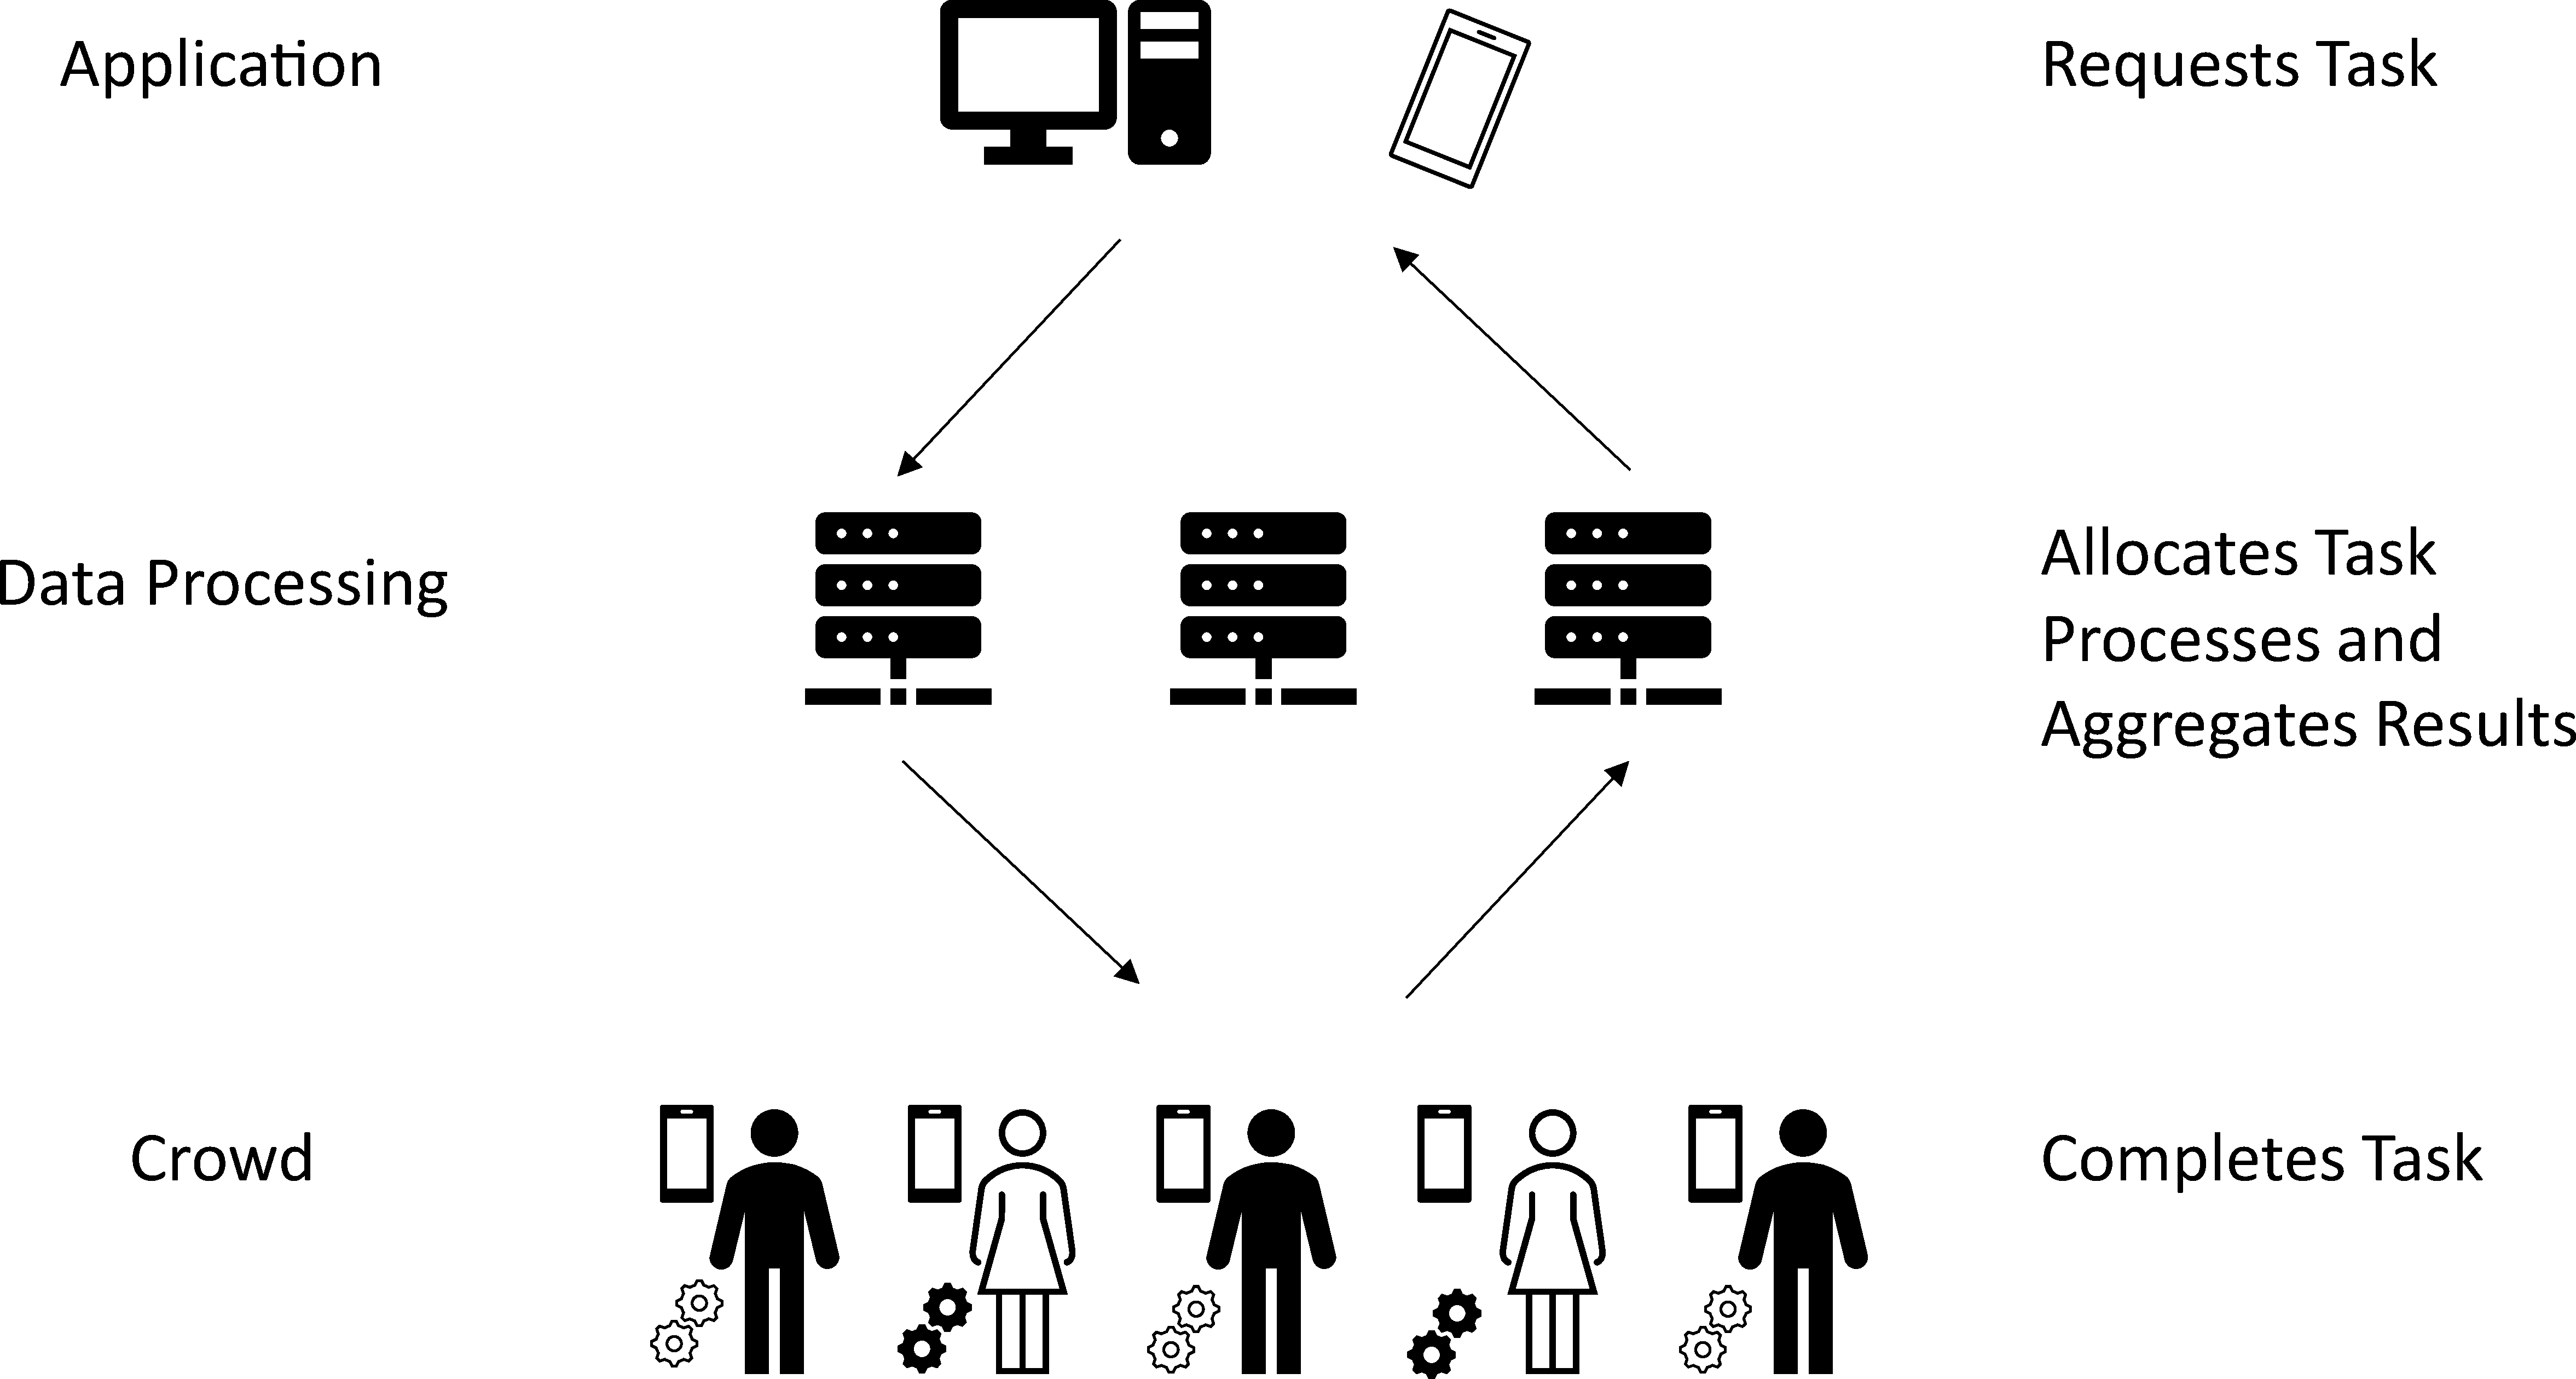
\includegraphics[width=0.8\textwidth]{fig/crowdsourcing.pdf}
  \caption{Crowdsourcing architecture consist of three layers: Application, Data Processing and Crowd}
  \label{fig:crowdsourcing_architecture}
\end{figure}

There are different aspects that characterize a crowdsourcing application: \textit{degree of human involvement}, \textit{location relevance}, \textit{knowledge requirement}, \textit{participation incentive}, and \textit{data flow}~\cite{ray2023survey,kong2019mobile}.

There are two types of \textit{degree of human involvement}: Opportunistic and Participatory.
The former describes that the participant does not actively operate the smartphone or device, while in the latter case, they have to give further input on the smartphone or device.
The \textit{degree of human involvement} is a continuum, where each crowdsourcing application can have different levels of human involvement.

\textit{Location relevance} refers to the importance of solving a task in a particular location.
With mobile crowdsourcing, a certain degree of \textit{location relevance} is naturally given, but there can still be different levels of \textit{location relevance}.
For instance, the task may need to be completely done at a specific location, or only parts of it, such as taking a photo of a location but then editing the photo anywhere.
Similar to the \textit{degree of human involvement}, here we also have a continuum, being between high location relevance and no location relevance at all.

\textit{Knowledge requirement} refers to the level of knowledge that the participant needs to fulfill a given task.
Some tasks may be very simple, where detailed knowledge is unnecessary, while other tasks may need some experts on a specific topic or extensive training to be able to solve the task.
A high \textit{knowledge requirement} may make it necessary to distinctively allocate the task to such participants, where the \textit{knowledge requirements} are met.

The \textit{participation incentive} can vary from project to project and also from participant to participant.
There are basically two types of incentives: intrinsic and extrinsic.
Participant with an intrinsic incentive engage with a crowdsourcing project, because they can identify with the problem the project wants to solve or simply enjoy performing the task.
There can also be extrinsic motivations such as getting paid or gaining social credits for it.
It is very much possible, that participants have both intrinsic \textit{and} extrinsic incentives to contribute to a project.

The \textit{data flow} is a technical aspect of the crowdsourcing project.
Here, there are three distinctions: centralized, decentralized, and hybrid.
When the data flows from the crowd directly to the processing platform, the project has a centralized data flow.
Contrary to that, when the data flow is decentralized, it means that some participants' devices collect the results of the solved tasks within the crowd and then send it in aggregated form to the processing platform.
This may be beneficiary to decrease the load on the processing platform.
A hybrid form is also possible, where the crowd or the crowd's devices process the data themselves and send it directly to the application, which makes the processing layer superfluous. 

\subsection*{Crowdsensing}
As in ``crowdsourcing'' the crowd in ``crowdsensing'' refers to a group of people, who voluntarily take over a task.
However, in crowd\textit{sensing}, the task at hand is mainly gathering data for the client, or in other words, \textit{sensing}.
Due to the similar nature of both, the architecture of crowdsensing projects is usually very similar to that of crowdsourcing projects (see Figure~\ref{fig:crowdsourcing_architecture}).
The main difference from a software architectural view is that the participants usually do not collaborate and thus there is no need for the smartphones and devices in the crowd to communicate with each other.

The characterization is also very similar, although there is usually no \textit{knowledge requirement} aspect in \textit{crowdsensing} projects.
However, there are two additional aspects, that can be used to characterize: \textit{application type} and \textit{data collection}.

There are mainly three \textit{application types}: environmental applications, infrastructure applications, and social applications~\cite{ganti2011mobile}.

In \textit{environmental applications}, the goal of the crowdsensing project is to gather data about the \textit{natural} environment.
Examples of \textit{environmental applications} are projects measuring air pollution~\cite{hasenfratz2012participatory,sivaraman2013hazewatch,liu2018third} or monitoring water quality~\cite{minkman2015citizen,rapousis2016performance,shang2023crowdwatersens}.

\textit{infrastructure applications} are about gaining insights into the state of public infrastructure.
Common use cases are gathering data about car parking spaces~\cite{villanueva2015crowdsensing,coric2013crowdsensing,rinne2014mobile} or traffic flow~\cite{wang2018city,li2019privacy,mei2020towards}.

As the name suggests, \textit{social applications} gather information about persons and social interactions.
With the help of social media networks, it is possible to extract information from the communications of the crowd~\cite{grasso2017public,cecilia2020mobile,phan2019drinks}, while there is also a focus on mass events~\cite{rahman2017location,cardone2014crowdsensing,jarvis2013ubicomp}.

The \textit{data collection} can come in two forms: \textit{mobile sensing} and \textit{user-generated}~\cite{pietschmann2008croco}.

In \textit{mobile sensing}, the smartphone or sensing device collects the data automatically.
The participant may need to start an app or turn on a device to start a recording of the sensor data.
When the smartphone or device that collects the data sends the collected data to the data processing platform autonomously, the data collection is \textit{push-based}, otherwise, if the data processing platform requests the collected data from an endpoint it is called \textit{pull-based}. 

\section{Citizen Science}
\label{sec:citizen_science_background}
Although the term Citizen Science was coined by Irwin~\cite{irwin2002citizen} and Bonney~\cite{bonney1996citizen} in the mid-90s, the concept is much older.
For example, the National Audubon Society's project called ``Christmas Bird Count'', where everyone is invited to participate in counting birds and report their findings, has run since the year 1900 and can be considered as the first Citizen Science project~\cite{silvertown2009new}.
This can be considered Citizen Science because it is a scientific endeavor, where anyone can participate, which is the broadest way to describe Citizen Science.
However, since the emergence of the term ``Citizen Science'', different definitions have been proposed by different scientific, social, and political parties~\cite{heigl2019toward,ecsa2015ten,us2016crowdsourcing} and there is an active discussion of what can be considered a Citizen Science Project and what cannot~\cite{haklay2021citizen}. 

Haklay et al.~\cite{haklay2021citizen} compiled a list of 32 definitions for Citizen Science from different reference sources, citizen science associations, global multinational organizations, and different governmental bodies.
One of their key findings is that although most definitions have descriptive, instrumental, and normative elements, the weighting can differ according to the goals of the proposing party of the definition.
\textit{National Geographic}, for example, has a more descriptive definition:
\begin{quotation}
\textit{``Citizen science is the practice of public participation and collaboration in scientific research to increase scientific knowledge. Through citizen science, people share and contribute to data monitoring and collection programs.''}~\cite{ullrich2024citizen}
\end{quotation}
After a broad description of what Citizen Science is, it underlines ``data monitoring and collection'' which is not surprising for an environmental-focused organization.

The \textit{National Institute of Environmental Health Sciences} chooses a more instrumentalist approach when defining Citizen Science:
\begin{quotation}
\textit{``Citizen science efforts are driven by community concerns. These community-led projects may involve a partnership with an academic or research institution, where both parties work together to collect and share data. The goal is to address a community concern through collaborative research and to translate the research findings into public health action that benefits the community.''}~\cite{national2022community}
\end{quotation}
The last sentence of their definition clearly puts a focus on public health, which is not understandable from their point of view.
There are also definitions that try to be normative, such as the definition from UNESCO:
\begin{quotation}
\textit{``[Citizen Science:] The participation of a range of non-scientific stakeholders in the scientific process. At its most inclusive and most innovative, citizen science involves citizen volunteers as partners in the entire scientific process, including determining research themes, questions, methodologies, and means of disseminating results.''}~\cite{vohland2021science}
\end{quotation}
It is remarkable that this definition mentions inclusiveness and voluntarism.

Eitzel et al.~\cite{eitzel2017citizen} also analyze different definitions of Citizen Science and identify three categories: Citizen Science as a \textit{tool}, a \textit{movement}, or a \textit{social capacity}.
Accordingly, Citizen Science can be seen as a \textit{tool} to help answer a research question, e.g. by gathering data.
On the other hand, Citizen Science can also be seen as a \textit{movement} to democratize science and thus increase the trust of society in science.
Finally, Citizen Science can be seen as a \textit{social capacity} to increase evidence-based decision-making.

The European Citizen Science Association~\footnote{https://www.ecsa.ngo/} contributes the ten principles of citizen science~\cite{ecsa2015ten}:

\begin{enumerate}
\item \textit{Citizen science projects actively involve citizens in scientific endeavour that generates new
knowledge or understanding. Citizens may act as contributors, collaborators, or as project
leader and have a meaningful role in the project.}
\item \textit{Citizen science projects have a genuine science outcome.} For example, answering a research
question or informing conservation action, management decisions or environmental policy.
\item \textit{Both the professional scientists and the citizen scientists benefit from taking part.} Benefits
may include the publication of research outputs, learning opportunities, personal enjoyment,
social benefits, satisfaction through contributing to scientific evidence e.g. to address local,
national and international issues, and through that, the potential to influence policy.
\item \textit{Citizen scientists may, if they wish, participate in multiple stages of the scientific process.} This may include developing the research question, designing the method, gathering and
analysing data, and communicating the results.
\item \textit{Citizen scientists receive feedback from the project.} For example, how their data are being used
and what the research, policy or societal outcomes are.
\item \textit{Citizen science is considered a research approach like any other, with limitations and biases
that should be considered and controlled for.} However unlike traditional research approaches,
citizen science provides opportunity for greater public engagement and democratisation of
science.
\item \textit{Citizen science project data and meta-data are made publicly available and where possible,
results are published in an open access format.} Data sharing may occur during or after the
project, unless there are security or privacy concerns that prevent this.
\item \textit{Citizen scientists are acknowledged in project results and publications.}
\item \textit{Citizen science programmes are evaluated for their scientific output, data quality, participant
experience and wider societal or policy impact.}
\item \textit{The leaders of citizen science projects take into consideration legal and ethical issues
surrounding copyright, intellectual property, data sharing agreements, confidentiality,
attribution, and the environmental impact of any activities.}
\end{enumerate}

The plethora of different definitions, guidelines, and principles show that Citizen Science is a broad term that can be interpreted according to the circumstances.
This, however, is also a benefit, since it allows different projects to label themselves as Citizen Science and get funding from different organizations and national institutions.

\section{Summary}
\label{sec:summary_background}
To summarize, there are four topics that we have described in this chapter.
Cycling comfort and cycling safety, which we introduced in the first two sections of this chapter, deal with factors that affect the comfort and safety during cycling.
These factors also reinforce or mitigate each other.
For example, a higher cycling safety, or rather the subjective perceiving of cycling safety, improves the cycling comfort.
And in reverse, a smooth cycling experience, e.g., achieved by a bicycle lane consisting of well-maintained, smooth tarmac, not only increases the cycling comfort, but also makes solitary accidents less likely and thus increases cycling safety.

In the second chapter we described Crowdsourcing and Crowdsensing, which are two ways of utilizing the ``crowd'' to achieve a goal.
In Crowdsourcing, the goal can be very diverse and the degree of the crowd's involvement can vary from simply be part of one step, or being involved in many tasks.
In contrast, Crowdsensing is usually limited to gathering data with the help of the crowd.
Finally, we focused on Citizen Science in the third section of this chapter.
There we discussed different perspectives on Citizen Science, that different research field and varying types of stakeholders such as the society, state institutions and research groups have.
Citizen Science can, depending on the use case, be utilized for different purposes, such as secure funding, attract more participants and help organize a project by giving a structure.

For a examination of the classification of our work with respect to the distinctions between crowdsourcing, crowdsensing, and citizen science, please refer to~\Cref{subsec:data_acquisition}.

%
%% There are MANY definitions. https://doi.org/10.1073/pnas.1909278116 and https://doi.org/10.5281/zenodo.3552753 compiled lists of them.
%% https://doi.org/10.5334/cstp.230 analyzed definitions.
%% Definitions have descriptive, instrumental, and normative aspects (https://link.springer.com/chapter/10.1007/978-3-030-58278-4_2#Sec2)
%% epistemology, methodology, and social practice and possible impacts on the given context of application.
%% aspects of citizen science: open data, open participation, voluntarity, open source, hierarchy
%% 5 types of citizen science projects: Action, Conservation, Investigation, Virtual, Education
%% 
%% From Citizen science: crowdsourcing for research Catherine Lichten
%% Citizen science projects also present an opportunity to involve non-researchers in the scientific process and for researchers to interact with the wider community. Involving the public in research can help to improve scientific understanding and literacy, and enhance public trust in science (Garbarino J., & C.E. Mason. 2016. ‘The Power of Engaging Citizen Scientists for Scientific Progress.’ Journal of Microbiology and Biology Education 17 (1): 7–12.)
%%
%% Three views on 'Citizen Science' (from Eitzel https://doi.org/10.5334/cstp.96):
%% 1) Instrumental, as a tool, method, or form of research collaboration  (e.g., Bonney et al. 2009b; Wiggins and Crowston 2011; Follett and Streznov 2015)
%% 2) a movement that democratizes the scientific research process (Irwin 1995)
%% 3) Social Capacity / knowledge-producing capacity of society and a path to evidence-based decision-making (Nielsen 2011)
%%
%% It is important to note that despite their reliance on micro-tasking and light engagement, there is evidence (Eveleigh et al. 2014) that some participants use the opportunity to develop deeper interest and engagement in science.
%%
%%
%%
%%
%%
%